\documentclass[12pt,a4paper]{article}
\usepackage{amsmath}
\usepackage{amssymb}
\usepackage{geometry}
\usepackage{parskip}  % Removes paragraph indentation and adds space between paragraphs
\usepackage{tikz}
\usepackage{xcolor}
\usepackage{hyperref}
\hypersetup{
    colorlinks=true,
    linkcolor=blue,
    urlcolor=blue,
    citecolor=blue,
    pdfborder={0 0 0},
}
\geometry{margin=1in}

% Set paragraph formatting
\setlength{\parindent}{0pt}
\setlength{\parskip}{0.8em}

% Aggressive widow and orphan control
\widowpenalty=10000  % Prevents single lines at the top of a page
\clubpenalty=10000   % Prevents single lines at the bottom of a page
\displaywidowpenalty=1000  % For math displays
\predisplaypenalty=10000    % Before displays
\postdisplaypenalty=10000   % After displays
\brokenpenalty=10000  % Penalty for page breaks after hyphenated lines
\interlinepenalty=10000  % Penalty between lines (for short paragraphs)

% Prevent section headings from appearing alone at bottom of page
\usepackage{needspace}  % Provides \needspace command
\usepackage[nobottomtitles*]{titlesec}  % Prevents section titles at bottom of page

% TikZ libraries
\usetikzlibrary{patterns,decorations.pathreplacing,calc,arrows.meta}

\begin{document}

\title{The Golden Ratio in Picture Framing:\\
\large A Mathematical and Historical Perspective}
\author{Matthias Nott\\
\small 1994, Translated and Critically Expanded, 2025}
\date{\today}
\maketitle

\begin{abstract}
This document presents a detailed mathematical derivation of the golden ratio and its application to the aesthetic problem of picture framing. We explore the concept of the ``optical center''---the visually pleasing vertical position of an image within a mat frame---and show how classical proportions can be adapted for practical use. Beyond the mathematics, we examine the historical context of measurement systems and provide a critical analysis of why the theoretical golden ratio must be modified for real-world application. The derivation reveals an elegant interplay between pure mathematics and human perception.
\end{abstract}

\section{Introduction: What is the Golden Ratio?}

The golden ratio, denoted by the Greek letter $\Phi$ (phi), has captivated human imagination for over two millennia. It appears throughout nature---in the spiral of nautilus shells, the arrangement of flower petals, and the proportions of the human body. Artists and architects have long recognized its aesthetic appeal, incorporating it into works from the Parthenon to the paintings of Leonardo da Vinci.

\subsection{Historical Context}

The golden ratio was first formally described in Euclid's \textit{Elements} (circa 300 BCE), Book II, Proposition 11, which states:

\begin{quote}
``To cut a given straight line so that the rectangle contained by the whole and one of the segments is equal to the square on the remaining segment.''
\end{quote}

In modern terms, we define the golden ratio as follows:

\begin{quote}
\textbf{Definition:} A line segment is said to be divided in the ``golden ratio'' when the ratio of the whole segment to the larger part equals the ratio of the larger part to the smaller part.
\end{quote}

\section{Mathematical Derivation of the Golden Ratio}

\subsection{Setting up the Problem}

Let's denote:

\begin{itemize}
    \item $M$ = the longer segment (called the ``Major'')
    \item $m$ = the shorter segment (called the ``Minor'')
    \item $M + m$ = the total length of the line segment
\end{itemize}

According to the definition, we have:

\begin{equation}
  \frac{\text{Total length}}{\text{Longer segment}} = \frac{\text{Longer segment}}{\text{Shorter segment}}
\end{equation}

Mathematically, this becomes:

\begin{equation}
  \frac{M + m}{M} = \frac{M}{m}
  \label{DefGold}
\end{equation}

\subsection{Solving for the Golden Ratio}

Let's solve equation (\ref{DefGold}) step by step to find the value of $\Phi = \frac{M}{m}$.

\textbf{Step 1:} Cross-multiply equation (\ref{DefGold}):
\begin{align}
  (M + m) \cdot m &= M \cdot M \\
  M \cdot m + m^2 &= M^2
\end{align}

\textbf{Step 2:} Divide both sides by $m^2$:
\begin{align}
  \frac{M \cdot m}{m^2} + \frac{m^2}{m^2} &= \frac{M^2}{m^2} \\
  \frac{M}{m} + 1 &= \left(\frac{M}{m}\right)^2
\end{align}

\textbf{Step 3:} Let $x = \frac{M}{m}$. Then we have:
\begin{align}
  x + 1 &= x^2 \\
  x^2 - x - 1 &= 0
\end{align}

\pagebreak

\textbf{Step 4:} Apply the quadratic formula where $a=1$, $b=-1$, $c=-1$:
\begin{align}
  x &= \frac{-b \pm \sqrt{b^2 - 4ac}}{2a} \\
  &= \frac{-(-1) \pm \sqrt{(-1)^2 - 4(1)(-1)}}{2(1)} \\
  &= \frac{1 \pm \sqrt{1 + 4}}{2} \\
  &= \frac{1 \pm \sqrt{5}}{2}
\end{align}

\textbf{Step 5:} Since we need $\frac{M}{m} > 0$ (both lengths are positive), we take the positive solution:

\begin{equation}
  \Phi \equiv \frac{M}{m} = \frac{1 + \sqrt{5}}{2} \approx 1.618033989...
  \label{Phi}
\end{equation}

This is the famous golden ratio!

\subsection{Properties of the Golden Ratio}

From our derivation, we can express the Major and Minor in terms of the total length:

\textbf{The Major (longer segment):}
Since $\frac{M+m}{M} = \Phi$, we can rearrange to get:

\begin{equation}
  M = \frac{M + m}{\Phi}
  \label{Major}
\end{equation}

\textbf{The Minor (shorter segment):}

\begin{align}
  m &= (M + m) - M \\
  &= (M + m) - \frac{M + m}{\Phi} \\
  &= (M + m)\left(1 - \frac{1}{\Phi}\right) \\
  &= (M + m)\left(\frac{\Phi - 1}{\Phi}\right)
  \label{Minor}
\end{align}

Interestingly, using $\Phi^2 = \Phi + 1$, we can show that $\Phi - 1 = \frac{1}{\Phi}$, so:

\begin{equation}
  m = \frac{M + m}{\Phi^2}
\end{equation}

\section{Visual Representation of the Concept}

Before diving into the application, let's visualize the difference between geometric centering and optical centering using diagrams.

\subsection{Geometric Center vs. Optical Center}

\begin{figure}[h!]
\centering
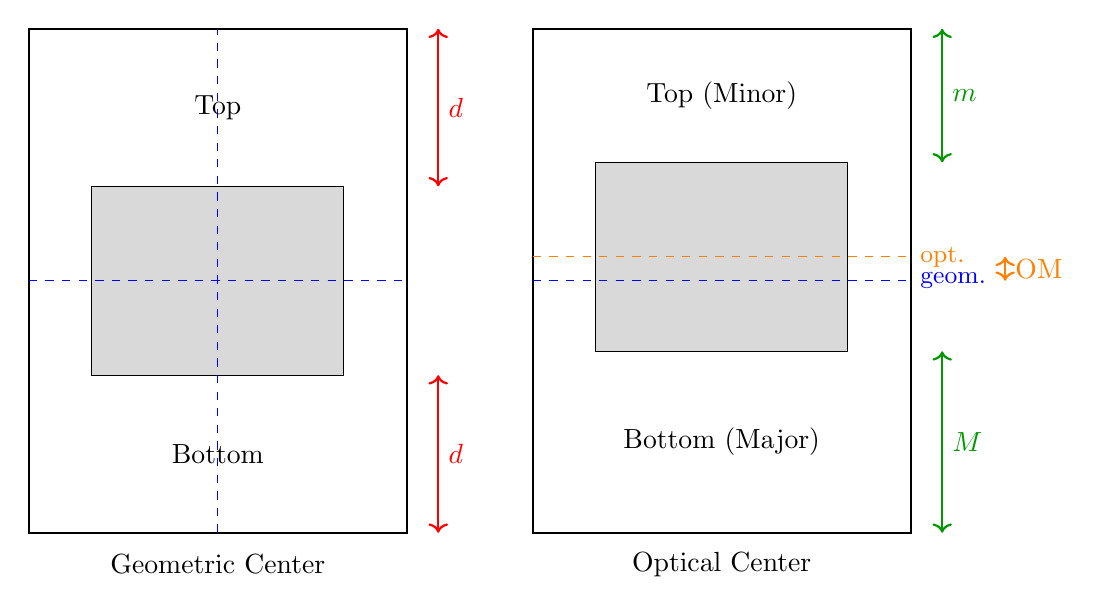
\begin{tikzpicture}[scale=0.8]
  % Left diagram - Geometrically centered
  \begin{scope}
    % Outer frame
    \draw[thick] (0,0) rectangle (6,8);
    \node at (3,-0.5) {Geometric Center};

    % Image (centered)
    \draw[fill=gray!30] (1,2.5) rectangle (5,5.5);

    % Dimension lines
    \draw[<->,red,thick] (6.5,0) -- (6.5,2.5) node[midway,right] {$d$};
    \draw[<->,red,thick] (6.5,5.5) -- (6.5,8) node[midway,right] {$d$};

    % Center lines
    \draw[dashed,blue] (0,4) -- (6,4);
    \draw[dashed,blue] (3,0) -- (3,8);

    % Labels
    \node at (3,1.25) {Bottom};
    \node at (3,6.75) {Top};
  \end{scope}

  % Right diagram - Optically centered
  \begin{scope}[xshift=8cm]
    % Outer frame
    \draw[thick] (0,0) rectangle (6,8);
    \node at (3,-0.5) {Optical Center};

    % Image (optically centered - higher)
    \draw[fill=gray!30] (1,2.88) rectangle (5,5.88);

    % Dimension lines
    \draw[<->,green!60!black,thick] (6.5,0) -- (6.5,2.88) node[midway,right] {$M$};
    \draw[<->,green!60!black,thick] (6.5,5.88) -- (6.5,8) node[midway,right] {$m$};

    % Center lines
    \draw[dashed,blue] (0,4) -- (6,4) node[right] {\small geom.};
    \draw[dashed,orange] (0,4.38) -- (6,4.38) node[right] {\small opt.};

    % OM arrow
    \draw[<->,orange,thick] (7.5,4) -- (7.5,4.38) node[midway,right] {OM};

    % Labels
    \node at (3,1.44) {Bottom (Major)};
    \node at (3,6.94) {Top (Minor)};
  \end{scope}
\end{tikzpicture}
\caption{Comparison of geometric centering (left) versus optical centering (right). In geometric centering, top and bottom margins are equal ($d = d$). In optical centering, the bottom margin $M$ is larger than the top margin $m$, creating a more visually balanced composition. The optical center (orange line) is higher than the geometric center (blue line) by the amount OM.}
\end{figure}

\subsection{The Golden Ratio Division}

\begin{figure}[h!]
\centering
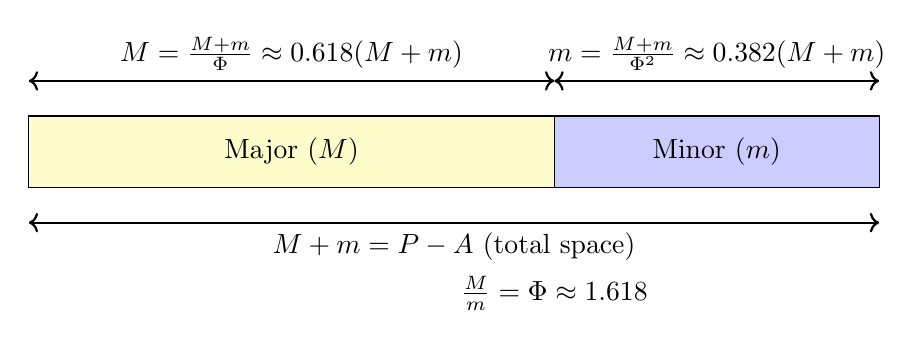
\begin{tikzpicture}[scale=0.9]
  % Total available space
  \draw[thick] (0,0) rectangle (12,1);
  \draw[fill=yellow!20] (0,0) rectangle (7.416,1);
  \draw[fill=blue!20] (7.416,0) rectangle (12,1);

  % Labels
  \node at (3.708,0.5) {Major ($M$)};
  \node at (9.708,0.5) {Minor ($m$)};

  % Dimensions
  \draw[<->,thick] (0,-0.5) -- (12,-0.5) node[midway,below] {$M + m = P - A$ (total space)};
  \draw[<->,thick] (0,1.5) -- (7.416,1.5) node[midway,above] {$M = \frac{M+m}{\Phi} \approx 0.618(M+m)$};
  \draw[<->,thick] (7.416,1.5) -- (12,1.5) node[midway,above] {$m = \frac{M+m}{\Phi^2} \approx 0.382(M+m)$};

  % Golden ratio indicator
  \node at (7.416,-1.5) {$\frac{M}{m} = \Phi \approx 1.618$};
\end{tikzpicture}
\caption{Division of available space according to the golden ratio. The total space $(P-A)$ is divided such that the ratio of Major to Minor equals $\Phi$.}
\end{figure}

\section{Application to Picture Framing}

\subsection{The Problem Statement}

When framing a picture, we face the aesthetic challenge of positioning an image of height $A$ within a mat (passepartout) of height $P$. The question is: how should we distribute the vertical space $P - A$ above and below the image?

For aesthetic reasons, the bottom margin should be larger than the top margin. This creates visual balance because:

\begin{itemize}
    \item It compensates for the optical illusion that makes centered objects appear lower than they actually are
    \item It provides visual stability, as we're accustomed to seeing more weight at the bottom
    \item It follows classical artistic proportions used in architecture and design
\end{itemize}

\subsection{Applying the Golden Ratio}

We apply the golden ratio to divide the available space $P - A$ into two parts:

\begin{itemize}
    \item Top margin = $m$ (the Minor)
    \item Bottom margin = $M$ (the Major)
\end{itemize}

where $M + m = P - A$.

\subsection{The Optical Center}

The ``optical center'' (OM) is defined as the difference between the bottom and top margins:

\begin{equation}
  \text{OM} \equiv M - m
  \label{OM}
\end{equation}

This represents how much higher the image should be placed from the geometric center of the frame (the image center is above the geometric center when the bottom margin is larger).

\subsection{Deriving the Formula for Optical Center}

Let's derive a practical formula for OM in terms of the total available space $(M + m)$.

\textbf{Step 1:} Substitute equations (\ref{Major}) and (\ref{Minor}) into (\ref{OM}):
\begin{align}
  \text{OM} &= M - m \\
  &= \frac{M + m}{\Phi} - (M + m)\left(1 - \frac{1}{\Phi}\right)
\end{align}

\textbf{Step 2:} Factor out $(M + m)$:
\begin{align}
  \text{OM} &= (M + m)\left[\frac{1}{\Phi} - \left(1 - \frac{1}{\Phi}\right)\right] \\
  &= (M + m)\left[\frac{1}{\Phi} - 1 + \frac{1}{\Phi}\right] \\
  &= (M + m)\left[\frac{2}{\Phi} - 1\right]
\end{align}

\textbf{Step 3:} Substitute $\Phi = \frac{1 + \sqrt{5}}{2}$:
\begin{align}
  \frac{2}{\Phi} - 1 &= \frac{2}{\frac{1 + \sqrt{5}}{2}} - 1 \\
  &= \frac{4}{1 + \sqrt{5}} - 1 \\
  &= \frac{4 - (1 + \sqrt{5})}{1 + \sqrt{5}} \\
  &= \frac{3 - \sqrt{5}}{1 + \sqrt{5}}
\end{align}

\textbf{Step 4:} Rationalize the denominator by multiplying by $\frac{1 - \sqrt{5}}{1 - \sqrt{5}}$:
\begin{align}
  \frac{3 - \sqrt{5}}{1 + \sqrt{5}} \cdot \frac{1 - \sqrt{5}}{1 - \sqrt{5}} &= \frac{(3 - \sqrt{5})(1 - \sqrt{5})}{(1 + \sqrt{5})(1 - \sqrt{5})} \\
  &= \frac{3 - 3\sqrt{5} - \sqrt{5} + 5}{1 - 5} \\
  &= \frac{8 - 4\sqrt{5}}{-4} \\
  &= \frac{4\sqrt{5} - 8}{4} \\
  &= \sqrt{5} - 2
\end{align}

Therefore:

\begin{equation}
  \text{OM} = (M + m)(\sqrt{5} - 2)
  \label{OM3}
\end{equation}

\needspace{8\baselineskip}
\section{The Practical Adjustment: Why Divide by Two?}

\subsection{The Theoretical vs. Practical Discrepancy}

In practice, the factor $(\sqrt{5} - 2) \approx 0.236$ proved to be too large for actual picture framing. This discrepancy arises from a fundamental difference between the theoretical model and the physical reality of framing.

\subsection{The Split Space Argument}

When I developed this formula in 1994, a key insight was that the golden ratio division is not applied to a continuous line segment, but rather to space that is split by the image itself. Consider:

\begin{itemize}
    \item In the classical golden ratio, we divide a single continuous line
    \item In picture framing, we have space above and below the image --- two separate regions
    \item The image acts as a visual interruption that fundamentally changes the perception
\end{itemize}

The argument for dividing by 2 can be understood as follows:

\begin{enumerate}
    \item The golden ratio creates an asymmetry of approximately 0.236 of the total space
    \item This asymmetry is distributed between two separate visual fields (above and below)
    \item Each field therefore receives half of the total asymmetry
    \item This results in the factor $\frac{\sqrt{5} - 2}{2} \approx 0.118$
\end{enumerate}

\subsection{Visual Explanation of the Division}

\begin{figure}[h!]
\centering
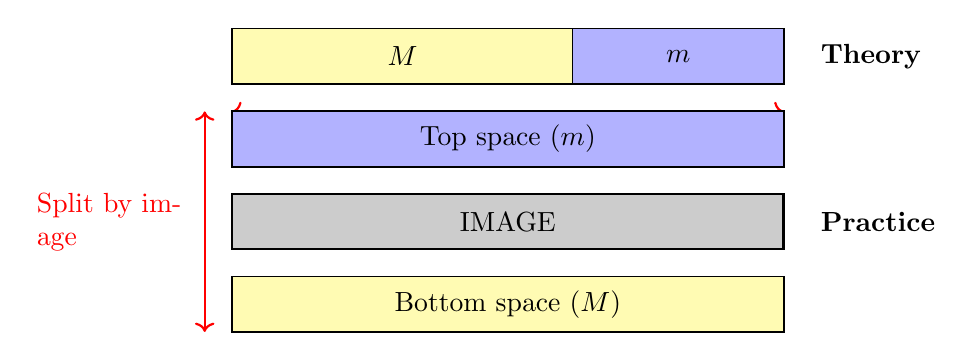
\begin{tikzpicture}[scale=0.7]
  % Theoretical continuous line
  \begin{scope}
    \draw[thick] (0,0) rectangle (10,1);
    \draw[fill=yellow!30] (0,0) rectangle (6.18,1);
    \draw[fill=blue!30] (6.18,0) rectangle (10,1);
    \draw[<->,thick,red] (0,-0.5) -- (10,-0.5) node[midway,below] {Continuous space};
    \node at (3.09,0.5) {$M$};
    \node at (8.09,0.5) {$m$};
    \node[anchor=west] at (10.5,0.5) {\textbf{Theory}};
  \end{scope}

  % Practical split space
  \begin{scope}[yshift=-4.5cm]
    \node[anchor=west] at (10.5,2) {\textbf{Practice}};
    % Top space
    \draw[thick] (0,3) rectangle (10,4);
    \draw[fill=blue!30] (0,3) rectangle (10,4);
    \node at (5,3.5) {Top space ($m$)};

    % Image
    \draw[thick,fill=gray!40] (0,1.5) rectangle (10,2.5);
    \node at (5,2) {IMAGE};

    % Bottom space
    \draw[thick] (0,0) rectangle (10,1);
    \draw[fill=yellow!30] (0,0) rectangle (10,1);
    \node at (5,0.5) {Bottom space ($M$)};

    % Annotations
    \draw[<->,thick,red] (-0.5,0) -- (-0.5,4) node[midway,left,text width=2cm] {Split by image};
  \end{scope}
\end{tikzpicture}
\caption{The theoretical model treats space as continuous, while in practice the image splits the space into two separate visual fields, justifying the division by 2.}
\end{figure}

\subsection{The Final Formula}

Through empirical testing and theoretical consideration, the final formula becomes:

\begin{equation}
  \boxed{\text{OM} = (P - A) \cdot \frac{\sqrt{5} - 2}{2} \approx (P - A) \cdot 0.118}
  \label{OM4}
\end{equation}

where:

\begin{itemize}
    \item $P$ = total height of the mat frame
    \item $A$ = height of the image cutout
    \item $\text{OM}$ = optical center offset (how much higher the image center should be from geometric center)
\end{itemize}

\needspace{10\baselineskip}
\section{Historical Context: Measurement Systems and Aesthetic Proportions}

\needspace{8\baselineskip}
\subsection{The Imperial-Metric Divide}

The application of mathematical proportions to practical crafts like picture framing highlights an interesting historical tension between measurement systems.

The golden ratio itself is a pure mathematical concept, independent of any measurement system. However, its practical application has been influenced by the tools and standards available to craftsmen throughout history:

\begin{itemize}
    \item \textbf{Ancient Systems:} The Greeks and Romans used body-based measurements (cubits, feet, digits) that naturally incorporated human proportions

    \item \textbf{Imperial System:} Evolved from these body-based measurements, often using fractions that approximate important ratios (e.g., 5/8 $\approx$ 0.625, close to $1/\Phi$)

    \item \textbf{Metric System:} Introduced during the French Revolution (1795) as a decimal system based on natural constants, emphasizing calculation over intuitive proportion
\end{itemize}

\needspace{8\baselineskip}
\subsection{The Craftsman's Dilemma}

Traditional framers often worked with rules of thumb rather than precise calculations:

\begin{itemize}
    \item ``Make the bottom margin 1/8 wider than the top'' (in inches)
    \item ``Add a thumb's width extra at the bottom''
    \item ``The bottom should be as the top plus the width of two fingers''
\end{itemize}

These approximations, while less mathematically precise, often produced results remarkably close to the golden ratio formula. This suggests that human aesthetic intuition naturally gravitates toward these proportions.

\needspace{8\baselineskip}
\subsection{Cultural Variations}

Different cultures have developed their own aesthetic standards for framing:

\begin{itemize}
    \item \textbf{Western tradition:} Emphasizes the bottom-heavy optical center
    \item \textbf{Japanese aesthetics:} Often uses asymmetrical placement following the rule of thirds
    \item \textbf{Islamic art:} Frequently employs geometric patterns that incorporate golden ratio spirals
\end{itemize}

\needspace{10\baselineskip}
\section{Critical Discussion}

\needspace{10\baselineskip}
\subsection{Is the Golden Ratio Truly Universal?}

While the golden ratio appears frequently in nature and art, its claimed universality deserves scrutiny:

\textbf{Arguments for universality:}

\begin{itemize}
    \item Appears in diverse natural phenomena (plant growth, DNA helices, galaxy spirals)
    \item Consistently rated as aesthetically pleasing in psychological studies
    \item Independently discovered by multiple cultures
\end{itemize}

\textbf{Arguments against universality:}

\begin{itemize}
    \item Many claimed instances are approximations or coincidences
    \item Cultural conditioning may influence aesthetic preferences
    \item Other ratios (like the silver ratio or root rectangles) also appear in art and nature
\end{itemize}

\needspace{10\baselineskip}
\subsection{The Division by Two: A Critical Analysis}

The decision to divide the golden ratio factor by two for picture framing deserves careful examination:

\textbf{Supporting arguments:}

\begin{enumerate}
    \item \textbf{Visual interruption:} The image creates a break in the visual field that fundamentally alters perception

    \item \textbf{Perceptual psychology:} The human eye processes separated spaces differently than continuous ones

    \item \textbf{Empirical validation:} Extensive practical testing confirmed the halved factor produces more pleasing results

    \item \textbf{Symmetry consideration:} The division distributes the asymmetry equally between two regions
\end{enumerate}

\textbf{Alternative interpretations:}

\begin{enumerate}
    \item \textbf{Center of gravity:} The adjustment might relate to how we perceive visual weight, with the image's center of gravity needing less offset than pure geometry suggests

    \item \textbf{Viewing angle:} Pictures are rarely viewed perfectly perpendicular; the adjustment might compensate for typical viewing angles

    \item \textbf{Frame thickness:} Physical frames add visual weight that might require compensatory adjustment
\end{enumerate}

\needspace{8\baselineskip}
\subsection{Limitations and Considerations}

The formula has several practical limitations:

\begin{itemize}
    \item Works best for rectangular frames with moderate aspect ratios
    \item May need adjustment for very tall or very wide images
    \item Digital displays might require different parameters than physical frames
    \item The formula assumes vertical orientation; horizontal layouts might need modification
\end{itemize}

\needspace{12\baselineskip}
\section{Practical Example}

Let's consider a concrete example with visual representation:

\begin{itemize}
    \item Mat frame height: $P = 50$ cm
    \item Image height: $A = 30$ cm
    \item Available space: $P - A = 20$ cm
\end{itemize}

Using formula (\ref{OM4}):
\begin{align}
  \text{OM} &= 20 \cdot \frac{\sqrt{5} - 2}{2} \\
  &\approx 20 \cdot 0.118 \\
  &\approx 2.36 \text{ cm}
\end{align}

This means:

\begin{itemize}
    \item The image center should be 2.36 cm above the geometric center of the frame
    \item Top margin: $\frac{20 - 2.36}{2} = 8.82$ cm
    \item Bottom margin: $\frac{20 + 2.36}{2} = 11.18$ cm
    \item Ratio of bottom to top margin: $\frac{11.18}{8.82} \approx 1.27$
\end{itemize}

\begin{figure}[h!]
\centering
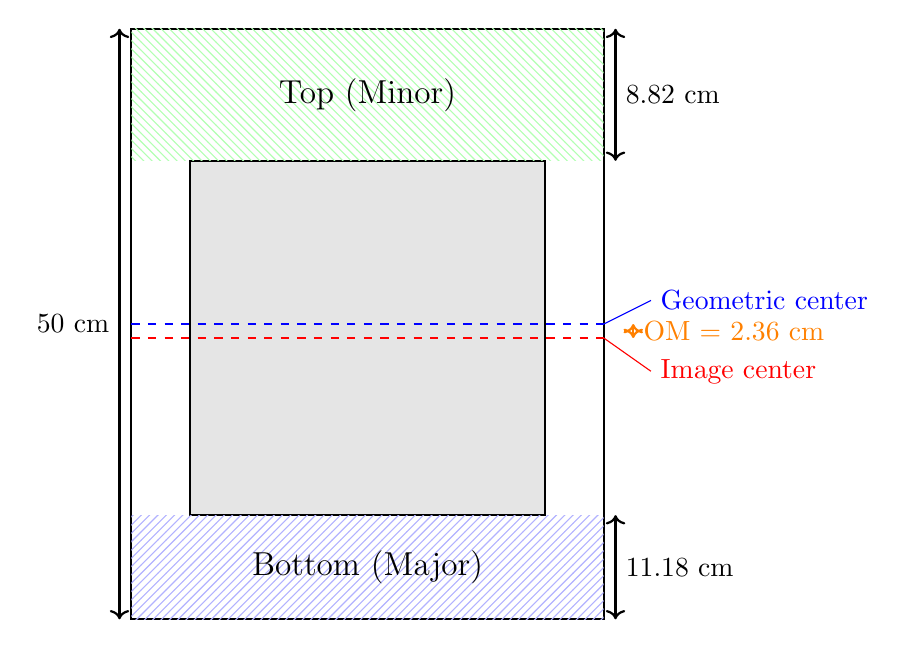
\begin{tikzpicture}[scale=0.15]
  % Frame
  \draw[thick] (0,0) rectangle (40,50);

  % Image
  \draw[thick,fill=gray!20] (5,8.82) rectangle (35,38.82);

  % Dimension arrows and labels
  \draw[<->,thick] (41,0) -- (41,8.82) node[midway,right] {11.18 cm};
  \draw[<->,thick] (41,38.82) -- (41,50) node[midway,right] {8.82 cm};
  \draw[<->,thick] (-1,0) -- (-1,50) node[midway,left] {50 cm};
  %\draw[<->,thick] (5,7.5) -- (35,7.5) node[midway,below] {Image};

  % Center lines
  \draw[dashed,blue] (0,25) -- (40,25);
  \draw[dashed,red] (0,23.82) -- (40,23.82);

  % Leader lines for labels
  \draw[blue] (40,25) -- (44,27) node[right] {Geometric center};
  \draw[red] (40,23.82) -- (44,21) node[right] {Image center};

  % OM indicator
  \draw[<->,thick,orange] (42.5,23.82) -- (42.5,25) node[midway,right] {OM = 2.36 cm};

  % Pattern for margins
  \pattern[pattern=north east lines, pattern color=blue!30] (0,0) rectangle (40,8.82);
  \pattern[pattern=north west lines, pattern color=green!30] (0,38.82) rectangle (40,50);

  \node at (20,4.41) {\large Bottom (Major)};
  \node at (20,44.41) {\large Top (Minor)};
\end{tikzpicture}
\caption{Practical example showing a 30 cm image in a 50 cm frame. The image center is positioned 2.36 cm above the geometric center, creating bottom margin of 11.18 cm and top margin of 8.82 cm.}
\end{figure}

Note that this ratio (1.27) is considerably less than the golden ratio itself (1.618), confirming that the halving adjustment creates a more subtle effect suitable for practical application.

\section{Conclusion}

The application of the golden ratio to picture framing represents a fascinating intersection of pure mathematics, aesthetic theory, and practical craft. The journey from Euclid's abstract geometric proposition to a concrete formula for mat cutting illustrates how mathematical principles can inform artistic practice.

The critical insight --- that the theoretical ratio must be halved for practical application --- reminds us that mathematical beauty must sometimes yield to perceptual reality. The split between upper and lower space, mediated by the image itself, creates a different visual experience than a continuously divided line segment.

This work demonstrates that while mathematics can provide valuable guidance for aesthetic decisions, the final arbiter must be the human eye and its complex perceptual apparatus. The formula presented here offers not a rigid rule but a starting point, a mathematically informed suggestion that framers can adjust based on specific circumstances and personal aesthetic judgment.

The enduring appeal of the golden ratio, whether in its pure or modified form, speaks to humanity's deep-seated desire to find order and beauty in proportion --- a quest that bridges cultures, centuries, and the eternal divide between theoretical ideals and practical realities.

\vspace{1cm}
\noindent\textit{Original Mathematical Work \copyright\ 1994--1995 Matthias Nott}\\
In Memoriam: My mother, Evi Arnholz, who founded Art \& Frame, a picture framing company in 1990 and inspired the younger me to this work and to the creation of the program OptiFrame. Both no longer exist...
\newline
\newline
\textit{Translation, Expansion, and Critical Analysis \copyright\ 2025 Matthias Nott}\\
Inspired by the great YouTube channel and video of \href{https://www.youtube.com/watch?v=bKMEDZp7ZZs}{Busted Knuckle Woodworks}

\end{document}